%
\documentclass[%
 reprint,
 amsmath,amssymb,
 aps,
]{revtex4-1}

\usepackage{graphicx}% Include figure files
\usepackage{dcolumn}% Align table columns on decimal point
\usepackage{bm}% bold math


\begin{document}



\title{Trabajo Final U I  \\ BOT Recomendacion de Framework para desarrollo de aplicaciones }
\author{Jhony Mamani Limache}
\author{Adnner Esperilla Ruiz}
\author{nombre}
\author{Marlon Villegas Arando}
\affiliation{%
 Universidad Privada de Tacna \textbackslash Facultad de Ingenieria \textbackslash Escuela Profesional de Ingenieria de Sistemas
}%

\begin{abstract}
\begin{center}
\textbf{Resumen}
\end{center}

En este artículo aprenderemos sobre la seguridad de los datos y lo que implica protegerlos de operaciones indebidas que pongan en peligro su definición, existencia, consistencia e integridad independientemente de la persona que los accede. Algunos comandos que se emplean para el objetivo del articulo es GRANT, REVOKE\\

\textbf{Palabras clave:}   seguridad, integridad, GRANT, REVOKE.\\

\begin{center}
\textbf{Abstract}
\end{center}
In this article we will learn about data security and what it means to protect data from improper operations that jeopardize its definition, existence, consistency and integrity regardless of who accesses it. Some commands used for the purpose of the article is GRANT, REVOKE\\
\textbf{Keywords:}   security, integrity, GRANT, REVOKE.\\

\end{abstract}



\maketitle

%\tableofcontents

\section {Introducción}\label{sec:1}





%-----------------------------------------------------------------
\section{Objetivos}\label{sec:2}
\subsection{General:}
-  Determinar como es que se establece la seguridad en las bases de datos.
\subsection{Específicos:}
-  Definir conceptos sobre seguridad de base de datos, privilegios y autorizaciones.\\
- Comparar las definiciones.

%-----------------------------------------------------------------
\section {Marco Teórico}

\subsection{¿Qué es seguridad de base de datos?}
\begin{itemize}
	\item La seguridad de los datos implica protegerlos de operaciones indebidas que pongan en peligro su definición, existencia, consistencia e integridad independientemente de la persona que los accede. Esto se logra mediante mecanismos que permiten estructurar y controlar el acceso y actualización de los mismos sin necesidad de modificar o alterar el diseño del modelo de datos; definido de acuerdo a los requisitos del sistema o aplicación software.
	\par El objetivo de la Seguridad de las Bases de Datos es proteger la Base de Datos contra accesos no autorizados. Se llama también privacidad. INCLUYE ASPECTOS DE:

	\subitem - Aspectos legales, sociales y éticos.
	\subitem - Políticas de la empresa, niveles de información pública y privada .
	\subitem - Controles de tipo físico, acceso a las instalaciones .
	\subitem - Identificación de usuarios: voz, retina del ojo, etc
	\subitem - Controles de sistema operativo.
	\item \textbf{TIPOS DE USUARIOS: } El DBA, tiene permitidas todas las operaciones, conceder privilegios y establecer usuarios:
	\subitem - Usuario con derecho a crear, borrar y modificar objetos y que además puede conceder privilegios a otros usuarios sobre los objetos que ha creado.
	\subitem - Usuario con derecho a consultar, o actualizar, y sin derecho a crear o borrar objetos.
	\item - Los SGBD tienen opciones que permiten manejar la seguridad, tal como GRANT, REVOKE, etc. También tienen un archivo de auditoria en donde se registran las operaciones que realizan los usuarios.
	\subitem - MEDIDAS DE SEGURIDAD
	\subitem - Físicas: Controlar el acceso al equipo. Tarjetas de acceso, etc.
	\subitem - Personal: Acceso sólo del personal autorizado. Evitar sobornos, etc.
	\subitem -SO: Seguridad a nivel de SO.
	\subitem - Herramientas de seguridad, perfiles de usuario, vistas, restricciones de uso de vistas, etc. \cite{web2}
	\item Un SMBD cuenta con un subsistema de seguridad y autorización que se encarga de garantizar la seguridad de porciones de la BD contra el acceso no autorizado.
	\subitem -Identificar y autorizar a los usuarios: uso de códigos de acceso y palabras claves, exámenes, impresiones digitales, reconocimiento de voz, barrido de la retina, etc  .
	\subitem -Autorización: usar derechos de acceso dados por el terminal, por la operación que puede realizar o por la hora del día.
	\subitem -Uso de técnicas de cifrado: para proteger datos en Base de Datos distribuidas o con acceso por red o internet. 
	\subitem - Diferentes tipos de cuentas: en especial del ABD con permisos para: creación de cuentas, concesión y revocación de privilegios y asignación de los niveles de seguridad.
	\subitem - Manejo de la tabla de usuarios con código y contraseña, control de las operaciones efectuadas en cada sesión de trabajo por cada usuario y anotadas en la bitácora, lo cual facilita la auditoría de la Base de Datos.
	\item \textbf{LAS TRES PRINCIPALES CARACTERÍSTICAS DE LA SEGURIDAD}  		\subitem -Que se deben mantener en una base de datos son la confidencialidad, la integridad y la disponibilidad de la información. 
	\subitem  -Los datos contenidos en una Base de Datos pueden ser individuales o de una Organización. \subitem -Sean de un tipo o de otro, a no ser que su propietario lo autorice, no deben ser desvelados. Si esta revelación es autorizada por dicho propietario la confidencialidad se mantiene. Es decir, asegurar la confidencialidad significa prevenir/ detectar/ impedir la revelación impropia de la información.
	
	
	
\end{itemize}


%-------------------------------------------------

\subsection{Principios básicos de la seguridad de base de datos}
\begin{itemize}
	\item \textbf{Identifique su sensibilidad: }Confeccione un buen catálogo de tablas o datos sensibles de sus instancias de base de datos. Además, automatice el proceso de identificación, ya que estos datos y su correspondiente ubicación pueden estar en constante cambio debido a nuevas aplicaciones o cambios producto de fusiones y adquisiciones.
	\par Desarrolle o adquiera herramientas de identificación, asegurando éstas contra el malware, colocado en su base de datos el resultado de los ataques de inyección SQL; pues aparte de exponer información confidencial debido a vulnerabilidades, como la inyección SQL, también facilita a los atacantes incorporar otros ataques en el interior de la base de datos.
	\item \textbf{Evaluación de la vulnerabilidad y la configuración: }Evalúe su configuración de bases de datos, para asegurarse que no tiene huecos de seguridad.
Esto incluye la verificación de la forma en que se instaló la base de datos y su sistema operativo (por ejemplo, la comprobación privilegios de grupos de archivo -lectura, escritura y ejecución- de base de datos y bitácoras de transacciones). Asimismo, con archivos con parámetros de configuración y programas ejecutables.
	\item \textbf{Endurecimiento: }Como resultado de una evaluación de la vulnerabilidad a menudo se dan una serie de recomendaciones específicas. Este es el primer paso en el endurecimiento de la base de datos. Otros elementos de endurecimiento implican la eliminación de todas las funciones y opciones que se no utilicen. Aplique una política estricta sobre que se puede y que no se puede hacer, pero asegúrese de desactivar lo que no necesita.
	\item \textbf{Audite: }Una vez que haya creado una configuración y controles de endurecimiento, realice auto evaluaciones y seguimiento a las recomendaciones de auditoría para asegurar que no se desvíe de su objetivo (la seguridad).
\par Automatice el control de la configuración de tal forma que se registre cualquier cambio en la misma. Implemente alertas sobre cambios en la configuración. Cada vez que un cambio se realice, este podría afectar a la seguridad de la base de datos.
	\item \textbf{Monitoreo: }Monitoreo en tiempo real de la actividad de base de datos es clave para limitar su exposición, aplique o adquiera agentes inteligentes de monitoreo, detección de intrusiones y uso indebido.
Por ejemplo, alertas sobre patrones inusuales de acceso, que podrían indicar la presencia de un ataque de inyección SQL, cambios no autorizados a los datos, cambios en privilegios de las cuentas, y los cambios de configuración que se ejecutan a mediante de comandos de SQL.
El monitoreo dinámico es también un elemento esencial de la evaluación de vulnerabilidad, le permite ir más allá de evaluaciones estáticas o forenses. Un ejemplo clásico lo vemos cuando múltiples usuarios comparten credenciales con privilegios o un número excesivo de inicios de sesión de base de datos.
	\item \textbf{Pistas de Auditoría: }Aplique pistas de auditoría y genere trazabilidad de las actividades que afectan la integridad de los datos, o la visualización los datos sensibles.
Recuerde que es un requisito de auditoría, y también es importante para las investigaciones forenses.
La mayoría de las organizaciones en la actualidad emplean alguna forma de manual de auditoría de transacciones o aplicaciones nativas de los sistemas gestores de bases de datos. 
	\item \textbf{Autenticación, control de acceso, y Gestión de derechos: }No todos los datos y no todos los usuarios son creados iguales. Usted debe autenticar a los usuarios, garantizar la rendición de cuentas por usuario, y administrar los privilegios para de limitar el acceso a los datos.
Implemente y revise periódicamente los informes sobre de derechos de usuarios, como parte de un proceso de formal de auditoría.
Utilice el cifrado para hacer ilegibles los datos confidenciales, complique el trabajo a los atacantes, esto incluye el cifrado de los datos en tránsito, de modo que un atacante no puede escuchar en la capa de red y tener acceso a los datos cuando se envía al cliente de base de datos. \cite{ff}

\end{itemize}

%-------------------------------------------------

\subsection{Medidas de seguridad y tipos de la seguridad de base de datos}
Las medidas de seguridad a considerar son las siguientes: 
\begin{itemize}
	\item \textbf{Físicas: }Comprenden el control de quienes acceden al equipo. 
	\item \textbf{Personal: }Determinación del personal que tiene acceso autorizado. 
	\item \textbf{Sistema Operativo: }Técnicas que se establecen para proteger la seguridad del Sistema Operativo. 
	\item \textbf{SGBD: }Utilización de las herramientas que facilita el SGBD. 
\end{itemize}
Existen dos tipos de mecanismos de seguridad de base de datos:
\begin{itemize}
	\item \textbf{Discrecional: }se usan para otorgar privilegios a los usuarios, incluida la capacidad de tener acceso a archivos, registros o campos de datos específicos en un determinado modo.
	\item \textbf{Obligatoria: }sirven para imponer igualdad de múltiples niveles clasificando los datos y los usuarios en varias clases (o niveles) de seguridad e implementando después la política de seguridad apropiada de la organización.
	\item Otra técnica de seguridad es el  \textbf{cifrado de datos}, que sirven para proteger datos confidenciales que se transmiten por satélite o por algún otro tipo de red de comunicaciones. El cifrado puede proveer protección adicional a secciones confidenciales de una base de datos \cite{l}
\end{itemize}
%-------------------------------------------------

\subsection{Requisitos para la seguridad de base de datos}
Para mantener la seguridad de la base de datos se necesita establecer controles para la protejan de futuros ataques extrenos, caídas o fallos del software o del equipo. Por ello, aquí se nombrará requisitos para tener un buen control de la seguridad de datos.
\begin{itemize}
\item La base de datos debe ser protegida contra el fuego, el robo y otras formas de destrucción.
\item Los servidores deben estar situados en un cuarto de accesso restringido para protegerlos y los administradores pueden tener acceso a estos desde un acceso remoto.
\item El administrador debe conocer distintos ataques que puede sufrir la base de datos y tratar de prevenirlos con anticipación.
\item Los datos deben ser reconstruibles, ya que siempre pueden ocurrir accidentes.
\item Se deben realizar copias de respaldo y estar constantemente actualizandolas para cuando se produzca errores de pérdida de datos.
\item Los datos deben poder ser sometidos a procesos de auditoria para cerciorarse de que todo se encuentre en orden o para descubrir si alguna persona ha accedido de manera ilegal o sin autorización.
\item El sistema debe diseñarse a prueba de intromisiones, no deben poder pasar por alto los controles.
\item Ningún sistema puede evitar las intromisiones malintencionadas, pero es posible hacer que resulte muy difícil eludir los controles.
\item El sistema debe tener capacidad para verificar que sus acciones han sido autorizadas.
\item Las acciones de los usuarios deben ser supervisadas, de modo tal que pueda descubrirse cualquier acción indebida o errónea.
\item Debe tomarse precaución acerca de cifrar los datos almacenados en la base de datos para protegerlos de los ataques que quieren acceder al sistema.  \cite{book1}
\end{itemize}
%-------------------------------------------------

\subsection{Características de la seguridad de base de datos}
El objetivo es proteger la base de datos contra los accesos no autorizados. Aqui 
\begin{itemize}
\item \textbf{Confidencialidad:} Se trata de la característica más importante de la seguridad de base de datos. Se logra a través del La encriptación que ha de aplicarse a datos en reposo, pero también a los datos que, por un motivo u otro, se encuentren en tránsito. \\ Por tanto, unicamente las personas que tengan la autorización correspondiete pueden acceder a la información almacenada.
\item \textbf{Integridad:} La Integridad es el término utilizado para decir que la información almacenada tiene calidad. El DBMS tiene que asegurar que los datos se almacenan de acuerdo a las políticas previamente determinadas por el DBA. \\ Consiste en mantener con exactitud la información tal como fue generada, sin ser manipulada o alterada por personas o procesos que no han sido autorizados.
\begin{center}
	\includegraphics[width=9cm]{./Imagenes/integridad}
\end{center}	
\item \textbf{Disponibilidad:} La información debe estar disponible para todos los usuarios con autorización en el momento que requieran.
\item \textbf{Concurrencia:} En algunos sistemas de ficheros, si hay varios usuarios que pueden acceder simultáneamente a un mismo fichero, es posible que el acceso interfiera entre ellos de modo que se pierda información o se pierda la integridad. La mayoría de los SGBD gestionan el acceso concurrente a la base de datos y garantizan que no ocurran problemas de este tipo.
\item \textbf{Recuperación:} Muchos sistemas de ficheros dejan que sea el usuario quien proporcione las medidas necesarias para proteger los datos ante fallos en el sistema o en las aplicaciones. Los usuarios tienen que hacer copias de seguridad cada día, y si se produce algún fallo, utilizar estas copias para restaurarlos. \cite{web1}
\end{itemize}
\begin{center}
	\includegraphics[width=7cm]{./Imagenes/imagen1}
\end{center}	
Garantizar la integridad en base de datos, así como su disponibilidad y confiabilidad es determinante para el buen funcionamiento del negocio. Sin embargo, la amenaza no da tregua y, a día de hoy, los ataques se multiplican, tanto en frecuencia, como en objetivo. \\\\  Los piratas informáticos ya no codician sólo los activos informacionales de las grandes corporaciones multinacionales, sino que tienen en su punto de mira a todo tipo de empresas, independientemente de su tamaño, propósito o industria.
%-------------------------------------------------

\subsection{Estrategias de la seguridad de base de datos}

\begin{itemize}
	\item Debido a que los archivos de registro de la base de datos pueden aumentar de tamaño entre una copia de seguridad y otra de SQL Server, realice una copia de seguridad diaria de la base de datos. Dependiendo de la frecuencia con que se ejecuten las actividades (tales como la generación de paquetes de informes y paneles de instrumentos, o trabajos de importación), se pueden realizar copias de seguridad incrementales frecuentes y copias de seguridad completas menos frecuentes. No es necesario realizar copias de seguridad mientras la base de datos está inactiva, pero se pueden planificar copias de seguridad para los momentos en que se sabe que la base de datos está menos ocupada. Si su empresa realiza un mantenimiento regular para servidores, este momento puede ser el mejor para realizar la copia de seguridad.
	\item Para empresas grandes en las que la base de datos nunca, o rara vez, está inactiva, puede utilizar software de copia de seguridad comercial que esté configurado para realizar copias de seguridad incrementales de SQL.\cite{oracle}

1.- Asignar de antemano el espacio necesario para los archivos de base de datos y archivos de registro puede mejorar el rendimiento.
 Estas opciones están disponibles en las páginas Archivos de datos y Registro de transacciones, en la ventana Propiedades de la base de datos de SQL Server Enterprise Manager.
\\
2.- Es necesario permitir que los archivos de registro aumenten de tamaño automáticamente  para asegurar que no se produzcan errores inesperados.
\\
3.- Colocar los archivos de datos y los archivos de registro en unidades de disco físicas separadas puede mejorar el rendimiento notablemente. Asegúrese de que estas unidades de disco físicas tengan suficiente espacio libre para permitir el crecimiento de la base de datos.

\end{itemize}


%-------------------------------------------------

\subsection{Importancia de la seguridad de base de datos}
\begin{itemize}
	\item Es importante desarrollar una política de seguridad para cada base de datos. La política de seguridad establece métodos para proteger su base de datos contra la destrucción accidental o malintencionada de datos o el daño a la infraestructura de la base de datos.
	\item Cada base de datos puede tener un administrador, conocido como el administrador de seguridad, quien es responsable de implementar y mantener la política de seguridad de la base de datos. Si el sistema de la base de datos es pequeño, el administrador de la base de datos puede tener las responsabilidades del administrador de la seguridad. Sin embargo, si el sistema de base de datos es grande, una persona designada o un grupo de personas puede tener la responsabilidad exclusiva como administrador de seguridad. \cite{oracle}
\end{itemize}
%-----------------------------------------------------------------
\section{INYECCIÓN SQL}
¿QUÉ ES LA INYECCIÓN SQL?
\begin{itemize}
\item El lenguaje de consulta estructurado, o SQL, es un método para administrar bases de datos relacionales que se concibió por primera vez en la década de 1970. Desde entonces, se ha convertido en el estándar en los sistemas de gestión de bases de datos (DBMS) y se puede encontrar en innumerables organizaciones de todo el mundo.
\item SQLi funciona, al menos en la superficie, de una manera muy directa: un atacante envía una declaración SQL maliciosa en un campo que se puede rellenar que explota una vulnerabilidad en la implementación de SQL de la aplicación web.
\begin{center}
	\includegraphics[width=7cm]{./Imagenes/1}
\end{center}	
\item Si tiene éxito, la declaración SQL maliciosa podría volcar todo el contenido de una base de datos, o seleccionar datos como registros de clientes, combinaciones de ID de empleado / contraseña, o cualquier otra cosa que contenga la base de datos seleccionada. SQLi también puede dar a un administrador de atacantes acceso a una base de datos, lo que les permite eliminar o modificar datos.
\begin{center}
	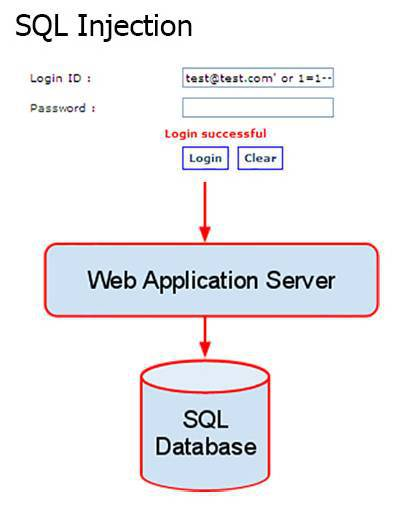
\includegraphics[width=7cm]{./Imagenes/2}
\end{center}	
	\item Los ataques de inyección SQL representan dos tercios de todos los ataques de aplicaciones web
Según los informes de Akamai, cuando se cuentan los ataques de inclusión de archivos locales, casi nueve de cada 10 ataques están relacionados con fallas de validación de entrada.
           \item Los ciberataques tienen varios vectores para acceder a las aplicaciones web, pero la inyección de SQL sigue siendo su opción más popular, según un nuevo análisis de datos de ataques.
           \item El ejercicio muestra que la inyección SQL (SQLi) ahora representa casi dos tercios   de todos Ataques de aplicaciones web. Eso se debe a la brusquedad de ataques en la  capa de aplicación web que SQLi representó hace solo dos años.
Los ataques de inclusión de archivos locales (LFI), que, como SQLi, también están habilitados por el hecho de que una aplicación web no haya validado correctamente los comentarios de los usuarios, representó otro 24.7 porciento de los ataques. En conjunto, los ataques SQLi y LFI representaron el 89.8 porciento de todos los ataques en la capa de aplicación .
- ¿Cuánta gente realmente entiende cómo escribir una aplicación que puede hablar de forma segura con la base de datos en el servidor?
 \item Pocos desarrolladores pueden entender la seguridad tan profundamente que una falla de seguridad realmente representaría un error para ellos.
\item  Los ataques SQLi clásicos son la forma más común y simple de SQLi.
\begin{center}
	\includegraphics[width=7cm]{./Imagenes/3}
\end{center}	

Los ataques clásicos pueden ocurrir siempre que una base de datos SQL permita a los usuarios enviar una declaración SQL. Vienen en dos variedades:

\item SQLi basado en errores, que consiste en hacer que una aplicación web arroje un error de SQL que proporciona al atacante información sobre la estructura de la base de datos o la información específica que está buscando
\item Ataques basados  en UNION que utilizan el operador sql union para determinar espetos especificos de la estructura de la base de datos con el fin de extraer informacion.
\item Los efectos de una inyección SQL exitosa pueden incluir:
\item Un atacante que crea una copia de la base de datos completa ;
\item un atacante suplantando las credenciales de inicio de sesión, haciéndose pasar por un usuario o incluso omitiendo la autenticación por completo;
\item modificación de la base de datos (por ejemplo, cambiar, eliminar o agregar registros);
\item robo de archivos que no pertenecen a la base de datos ubicados en el sistema de archivos de la DMBS;
\item ejecución de comandos del sistema operativo que le dan al atacante acceso a otros activos en la red que hospeda la base de datos SQL; y llamando a la aplicación web de destino / DBMS fuera de línea.

\end{itemize}
%-----------------------------------------------------------------
\section{Análisis}

\begin{itemize}
	\item Es necesario conocer los diferentes ataques que puede sufrir una base de datos y tratar de prevenirlos con anticipación. 
	\item Las bases de datos SQL almacenan información crítica y, a pesar de eso, muchos sitios web siguen siendo vulnerables a los ataques de SQLi, como aquellos que apuntan a SQL, que siguen siendo el riesgo de seguridad de la aplicación web más importante.
\end{itemize}
%-----------------------------------------------------------------
\section{Conclusiones}

\begin{itemize}
	\item La seguridad de los datos implica protegerlos de operaciones indebidas que lo pongan en peligro, esto se logra mediante mecanismos que permiten estructurar y controlar el acceso y actualización de los mismos sin necesidad de modificar o alterar el diseño del modelo de datos.
	\item Aunque realizar la implementación de la seguridad más sofisticada no es tarea fácil, debemos hacer el esfuerzo de lograr que los datos estén completamente seguros para el bien de la información de las organizaciones, empresas, entre otros.
           \item La seguridad de la base de datos es uno de los temas más Importantes para los DBA y uno de los aspectos más importantes de su función ya que  con los crecientes riesgos de los ataques cibernéticos, los cortes de bases de datos y las fugas de datos, es esencial saber cómo habilitar y aprovechar al máximo todas las características de seguridad .
           \item A pesar de tener muchas herramientas para la seguridad de base de datos es crucial que, al momento de aplicar alguna de estas, debe ser con estrategia, según las condiciones que está implicando. Ya que alguna mala decisión no servirá el método con el cual se esta protegiendo una Base de Datos
\end{itemize}


% Bibliografia.
%-----------------------------------------------------------------

\bibliographystyle{plain}
\bibliography{Bibliografia}

\end{document}
